\documentclass{standalone}

\usepackage{fontspec}
\usepackage[dvipsnames]{xcolor}
\usepackage{tikz}
\usepackage[skins]{tcolorbox}

\definecolor{paper}{HTML}{F1EBDB}

\usepackage{eso-pic}

\begin{document}
%\pagecolor{paper}
%\AddToShipoutPictureBG{
%	\begin{tikzpicture}[remember picture, overlay]
%		\draw[fill stretch image=Images/paper_texture_vertical.png]  (current page.south west) rectangle (current page.north east);
%	\end{tikzpicture}
%}
\begin{tikzpicture}
%\setmainfont[Scale=2.0]{Grizzly Attack}
%\huge
%%\node[inner sep=0pt] at (0,3.75cm) {Kill the Beast ?};
\node[inner sep=0pt, fill overzoom image=Images/paper_texture_vertical.png, minimum height=10cm, minimum width=12.6cm] at (0cm,0cm) {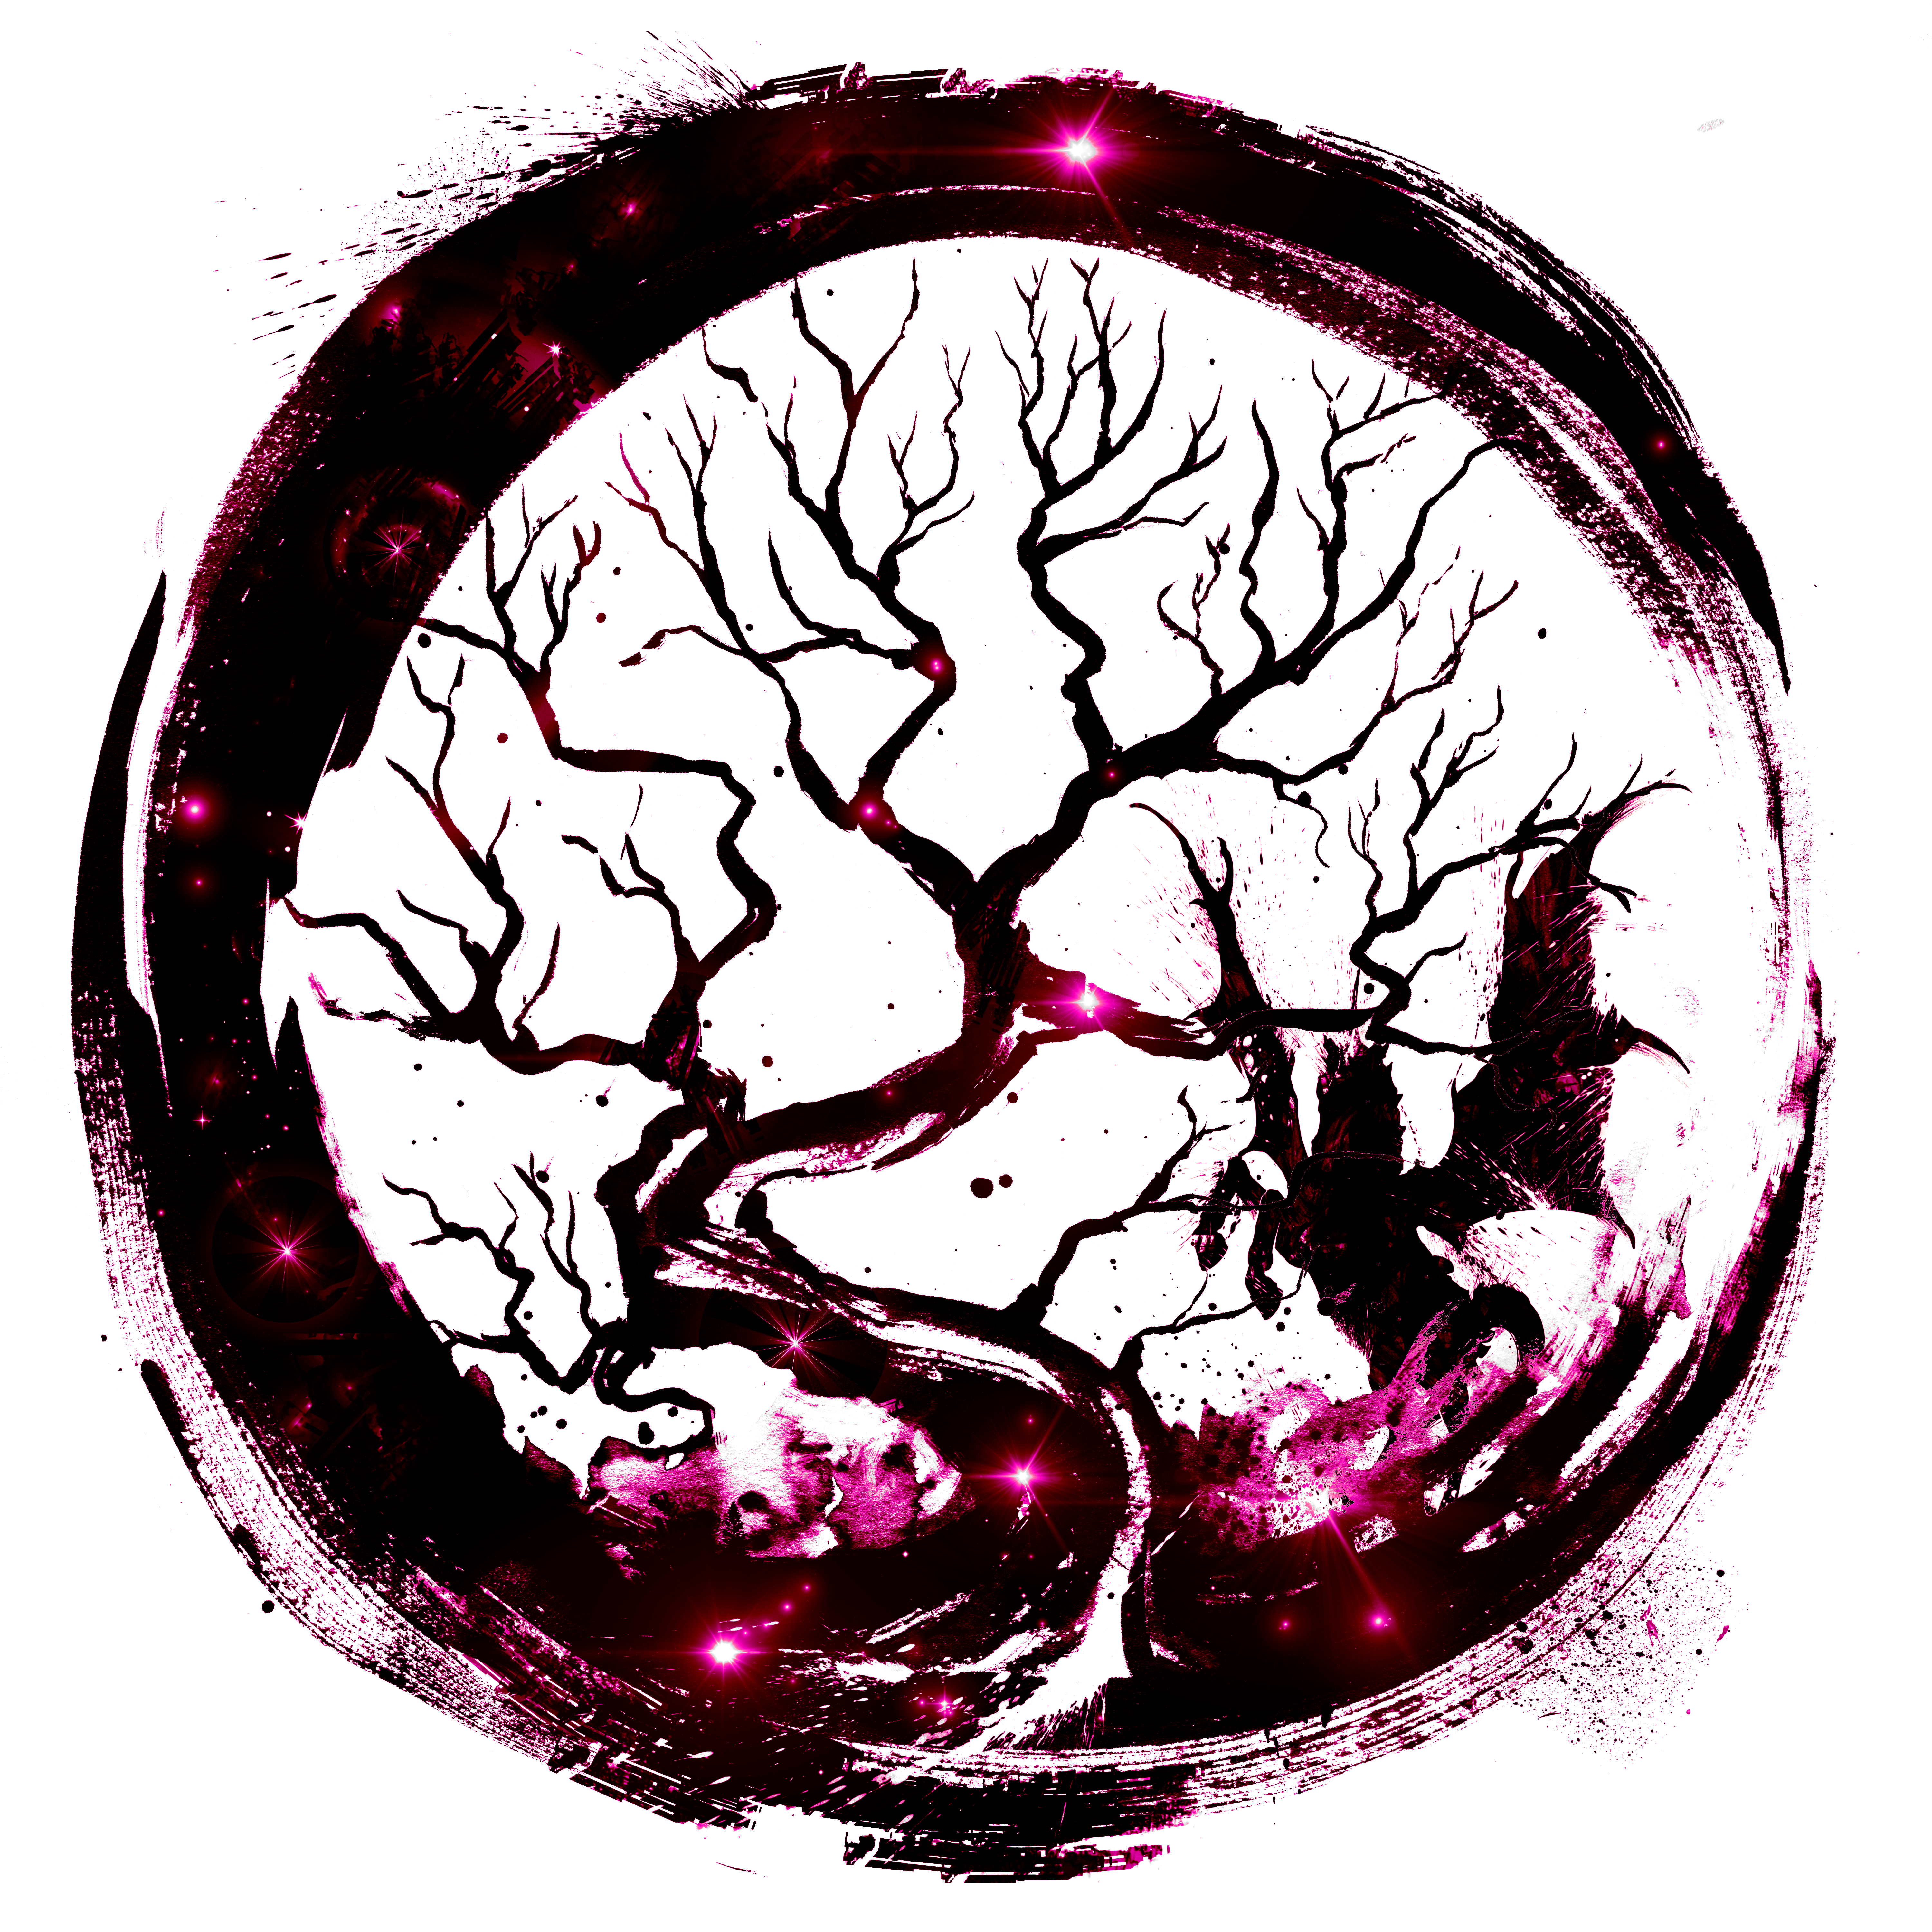
\includegraphics[scale=0.1825]{Images/kill_the_beast_cover_image_purple.png}};
%\setmainfont{Water Brush}
%\LARGE
%\node[inner sep=0pt] at (0,-4.125cm) {A Scoratic Worldbuilding Game by Michael Purcell};
%\node[fill overzoom image=Images/paper_texture_vertical.png, minimum height=10cm, minimum width=12.6cm] at (0,0) {};
\path (-6.3cm, -5cm) -- (6.3cm, 5cm);
\end{tikzpicture}

\end{document}